\section{Introduzione}
\subsection{Preparazione dell'apparato sperimentale}

Per questa esperienza è d'obbligo prestare una particolare attenzione alla costruzione dell'apparato sperimentale, in quanto anche piccole dimenticanze o imprecisioni possono causare variazioni notevoli nelle misurazioni.
Si proceda quindi con la preparazione dell'apparato: versare un pò d'acqua nel contenitore, posarlo sopra l'agitatore magnetico ed inserire l'ancoretta magnetica al suo interno; controllare quindi che l'agitatore magnetico faccia vibrare l'ancoretta che, a sua volta, deve garantire la rotazione dell'acqua che la circonda.
Questa prima verifica è necessaria in quanto l'acqua diventerà il bagno termico per tutta la durata dell'esperimento e quindi il mescolamento dell'agitatore termico è una condizione necessaria per l'omogeneità dell'acqua che andrebbe, in sua assenza, a stratificarsi in base alla sua temperatura.
Controllare quindi che l'interno della bottiglia contenente il gas non sia in nessun modo bagnato e, tenendo aperti i rubinetti, fissarla stabilmente all'apposito sostegno in modo che essa possa resistere alla spinta idrostatica ed in modo da permettere il funzionamento dell'agitatore magnetico.
Collegare quindi un ramo del manometro ad uno dei rubinetti della bottiglia ed, aiutandosi con la siringa di plastica, versare acqua nel manometro tenendo i due rami del manometro alla stessa altezza e prestando particolare attenzione in modo da evitare la formazione di bolle d'aria.
Riempire il più possibile il manometro con acqua, prestando attenzione che l'acqua raggiunga il più alto livello possibile non superando la parte rigida trasparente, grazie alla quale riusciremmo a prendere le misure sulla scala millimetrata posta accanto.
Verificare nuovamente che la bottiglia contenente il gas sia perfettamente asciutta.

\subsection{Termalizzazione iniziale dell'aria}
Procedere quindi con la termalizzazione dell'aria.
Preparare il bagno termico intorno alla bottiglia e tramite il termometro controllare l'uniformità della temperatura, garantita dall'agitatore termico.
Scegliamo di termalizzare inizialmente intorno ai $0^{\degree}$ C per poi salire fino ad una temperatura di circa $20^{\degree}$ C e quindi ridiscendere nuovamente fino al valore iniziale.
Scegliendo questa procedura di misurazione la bottiglia si troverà sempre in sovrapressione rispetto alla pressione atmosferica: in questo caso quindi il manometro dovrà essere montato sul tavolo con il lato libero in grado di salire di circa 80 cm sopra la posizione iniziale.
Scegliendo di termalizzare il sistema a $0^{\degree}$ C la presenza di ghiaccio nel bagno dovrà essere presente in maniera predominante rispetto all'acqua: la coesistenza di queste due fasi assicura che la temperatura sia uguale allo zero termico.
Immergere quindi la bottiglia nel bagno termico fino al tappo, prestando attenzione che non raggiunga i giunti di connessione dei rubinetti: in questo modo permetteremo una migliore termalizzazione del gas.
Una volta raggiunto l'equilibrio termico alla temperatura iniziale prescelta, aprire il rubinetto e richiuderlo: in questo modo la pressione del gas all'interno della bottiglia viene uniformata con la pressione atmosferica $P_{A}$.
Dopo la ciusura del rubinetto il volume e le moli del gas rimarranno costanti per tutta la durata dell'esperimento.
Procediamo quindi con le misurazioni.\\

\subsection{Procedura di misurazione}
Come già affermato, scegliamo di termalizzare inizialmente intorno ai $0^{\degree}$ C per poi salire fino ad una temperatura di circa $20^{\degree}$ C e quindi ridiscendere nuovamente fino al valore iniziale.
Per aumentare la temperatura del bagno di fusione, procediamo sostituendo gradualmente l'acqua del recipiente con acqua più calda; al contrario, per diminuire la temperatura del bagno di fusione, procediamo sostituendo gradualmente l'acqua del recipiente con acqua di fusione e ghiaccio.
Ad ogni variazione di temperatura bisogna riportare il valore del volume del gas al valore iniziale, andando ad alzare o abbassare il ramo libero del manometro.
Andando a incrementare o diminuire la pressione della colonnina d'acqua che preme sul ramo libero del manometro, si va ad incrementare o diminuire la pressione del gas nell'ampolla che permetterà quindi al gas di tornare al suo volume iniziale.
Aspettare un tempo sufficiente per permettere che il gas nell'ampolla ed il bagno siano all'equilibrio termico e prendere quindi le misure di temperatura $T$ e di dislivello $\Delta h = h_1 - h_0$, dove $h_0$ è la posizione iniziale e $h_1$ è l'altezza a cui è stato alzato il ramo libero del manometro.
Abbiamo ripetuto tutta questa procedura due volte, andando quindi a raccogliere due set di dati che verranno analizzati separatamente e poi confrontati per riuscire a apprezzare eventuali errori sistematici nelle misure.
\\
Con questa procedura di misura le incertezze del dislivello che abbiamo sono esclusivamente di risoluzione:
\begin{equation}
\sigma (\Delta h) = \sqrt{(\sigma h_1)^2 + (\sigma h_0)^2} = \frac{\Delta X}{\sqrt{6}}
\end{equation}
dove con $\Delta X$ indichiamo il la risoluzione del metro, pari a $0.1$ cm.
Troviamo quindi una incertezza sulle misurazioni di dislivello pari a $\sigma (\Delta h) = 0.04$ cm .
Per quando riguarda l'incertezza sulle misure di temperatura otteniamo invece una incertezza di risoluzione pari a $\sigma T = \frac{0.1}{\sqrt{12}}$ $^{\degree}$ C,infatti abbiamo scelto di non considerare l'ultima cifra del termometro per varie motivazioni: prima tra tutte quella che questa cifra non era per niente stabile, ma continua ad oscillare tra più valori; la seconda è che questa cifra era relativa alla temperatura di un singolo punto, ovvero il punto in cui il termometro misurava la temperatura del bagno termico, mentre a noi interessava una misura più generale.
Per questo decidiamo di non considerare questa ultima cifra dell'ordine di $0.01^{\degree}$ C relativa alla misura di temperatura in quanto considerata non significativa e poco rilevante per questo esperimento.

\subsection{Pressione assoluta}
Durante tutta la durata dell'esperienza di laboratorio si deve tenere conto di una grandezza, la pressione atmosferica $P_A$, che non è costante nel tempo.
È quindi necessario tenere una traccia oraria relativa alle misurazioni effettuate ed anche prendere numerose misurazione della pressione atmosferica nell'arco temporale dell'esperienza.
Per effettuare queste misurazioni adoperiamo il barometro situato nel laboratorio.
La pressione $P$ del gas nell'ampolla si ottiene:
\begin{equation}
P = P_A + \rho g h
\end{equation}
dove $P_A$ è la pressione atmosferica calcolata con il barometro, $\rho = 1 \frac{kg}{dm^3}$ è la densità dell'acqua e $g = 9.807 \frac{m}{s^2}$
è l'accelerazione di gravità.
L'incertezza su questa misura è data dalla risoluzione del barometro, ovvero $\sigma P = 39.98$ Pa.

\section{Analisi dati: primo set}
\subsection{Pressione e temperatura}

\begin{table}[H]
\centering
	\begin{subtable}{.5\textwidth}
		\centering
		\begin{tabular}{|c|c|} \hline
			\textbf{$\Delta h {[cm]}$ } & \textbf{T {[\degree C]} }  \\ \hline
			0 & 0  \\ \hline
			8.5 & 2.3  \\ \hline
			15.9 & 4.1  \\ \hline
			24 & 6.1  \\ \hline
			31.7 & 8.1  \\ \hline
			40.4 & 10  \\ \hline
			49.8 & 12.1  \\ \hline
			56.8 & 14.3  \\ \hline
			63.3 & 16  \\ \hline
			71.8 & 18.4  \\ \hline
			77.6 & 20  \\ \hline
		\end{tabular}
		\caption{Aumento della temperatura }
	\end{subtable}%
	\begin{subtable}{.5\textwidth}
	\centering
	\begin{tabular}{|c|c|} \hline
		\textbf{$\Delta h {[cm]}$ } & \textbf{T {[\degree C]} }  \\ \hline
		77.6 & 20  \\ \hline
		73.4 & 18.8  \\ \hline
		66.2 & 17  \\ \hline
		59.4 & 15  \\ \hline
		52.4 & 13.1  \\ \hline
		44.2 & 11  \\ \hline
		36.2 & 8.9  \\ \hline
		26.5 & 6.9  \\ \hline
		18.9 & 5.1  \\ \hline
		-0.5 & 0  \\ \hline
	\end{tabular}
	\caption{Diminuzione della temperatura }
\end{subtable}

\caption{Dislivello $\Delta h$ in funzione della temperatura $T$ }
\end{table}
In Tabella 1.a e Tabella 1.b troviamo riportati il primo set di dati raccolti durante la nostra esperienza rispettivamente aumentando e diminuendo la temperatura del bagno termico.
Troviamo graficati tali dati in Figura 1. 

\begin{figure}[H]
\centering
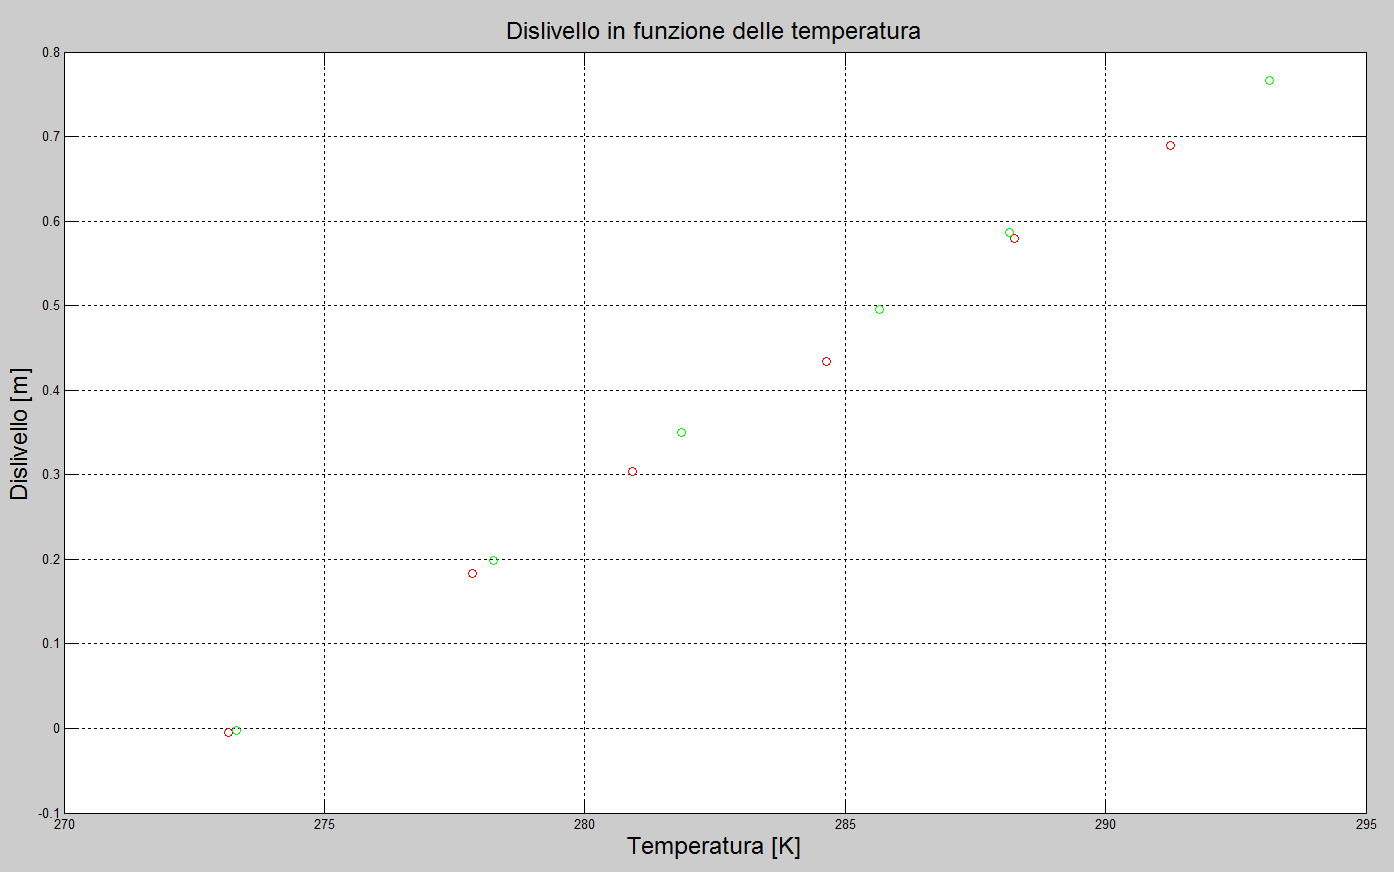
\includegraphics[width=\textwidth]{img/1}
\caption{Grafico di $\Delta h$ in funzione di $T$: in colore rosso i dati riportati in Tabella 1.a ed in colore verde i dati riportati in Tabella 1.b }
\end{figure}

Tramite regressione lineare troviamo la retta $h = A+BT$ che meglio interpreta i nostri dati. 
Per farlo dobbiamo innanzitutto trasferire le incertezze dalle ascisse alle ordinate, procediamo quindi a stimare graficamente un valore iniziale della pendenza $B$ della retta e trasferiamo l'incertezza.
\begin{equation}
\label{eq:propagazione}
\sigma(\Delta h)_{tot} = \sqrt{\sigma(\Delta h)^2 + (B\sigma T)^2}
\end{equation}
Le formule per il calcolo sono la \eqref{eq:a} e la \eqref{eq:b} riportate in Appendice A. 
Otteniamo:
\[A = -10.73 \pm 0.01 m \quad  B = 0.0393 \pm  0.00004 \frac{m}{K} \] .
Verifichiamo la bontà di questo risultato tramite test del $\chi^2$. 
Ci viene un $\chi^2 = 948.6366$, decisamente troppo alto come valore.
La retta quindi interpreta malamente i nostri dati. 
In Figura 1 si può osservare come i vari dati non siano allineati sulla retta. 
Sempre in Figura 1 possiamo osservare come i nostri dati si comportino in maniera diversa sopra e sotto i 285 K. 
Infatti questa è circa la temperatura di rugiada dell'aria. 
Ci aspettiamo quindi che al di sopra di questa temperatura l'aria si comporti come un gas ideale mentre al di sotto ci sarà un contributo dato dal vapore che sarà pari alla tensione di vapor saturo; avremmo quindi una più forte pendenza in funzione della temperatura in quanto la tensione di vapore saturo mostra derivata rispetto alla temperatura maggiore rispetto a quella del gas perfetto.\\
\newline
Dividiamo quindi i dati in due parti, divise dalla temperatura di rugiada 285 K.

\begin{figure}[H]
\centering
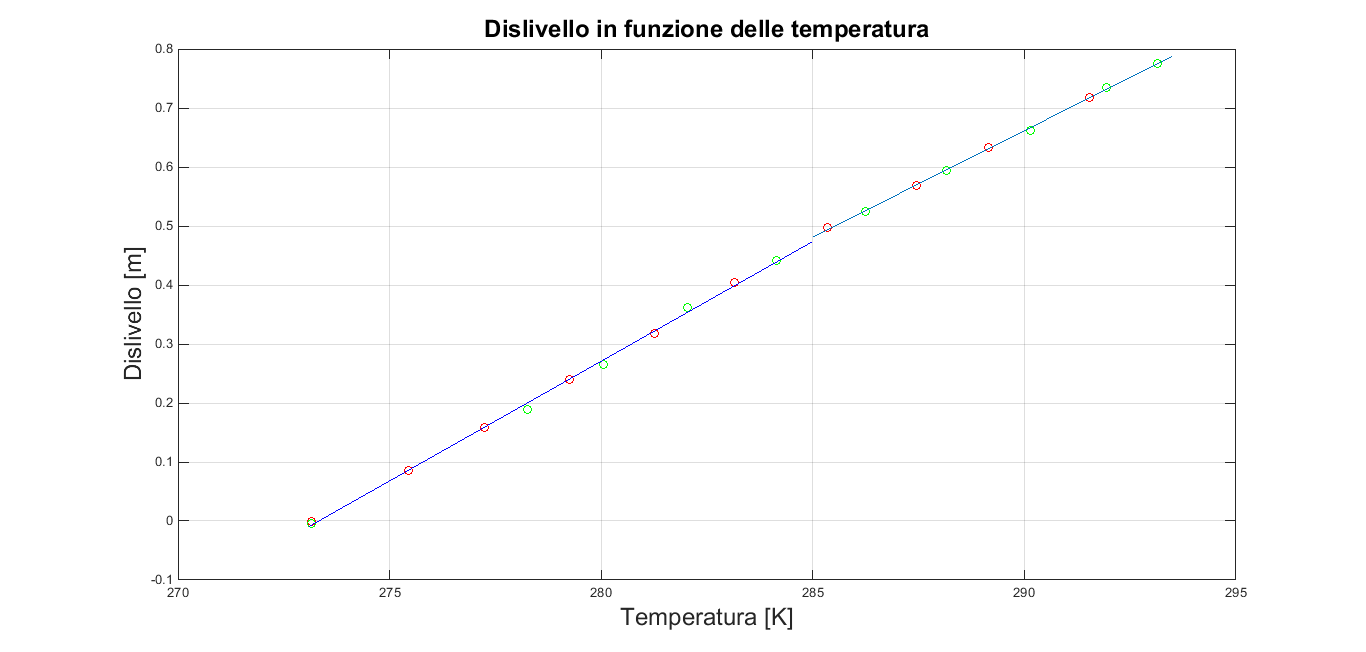
\includegraphics[width=\textwidth]{img/2}
\caption{Grafico di $\Delta h$ in funzione di $T$: 2 rette diverse per i dati divisi da 285 K}
\end{figure}

Iniziamo a valutare i dati al di sotto dei 285 K.\\
Procediamo nello stesso identico modo usato precedentemente e tramite regressione lineare troviamo la retta $h = A+BT$.
Otteniamo:
\[A = -11.09 \pm 0.03 m \quad  B = 0.0406\pm 0.0001 \frac{m}{K}\]
Otteniamo un $\chi^2$ pari a 231.5047. 
Il valore del $\chi^2$ risulta ancora troppo alto, molto probabilmente perchè abbiamo sottostimato le incertezze sui valori.
Procediamo quindi calcolando le incertezze a posteriori:
\begin{equation}
\label{eq:post}
\sigma(\Delta h)_{post} = \frac{1}{N-2}\sum_{i=1}^N(h-A-BT)^2
\end{equation}
Otteniamo una incertezza a posteriori pari a $6.3$ mm. 
È piuttosto difficile attribuire questa incertezza alla lettura della scala graduata del metro: ad essa contribuisce infatti anche la risoluzione del termometro che non basta però a spiegarla completamente. 
Per comprenderne il significato dobbiamo considerare la variazione di pressione atmosferica $P_A$ durante la sessione in cui sono state prese le misure. 
Questa analisi iniziale non tiene conto del suo effetto che è però già ben visibile in questa incertezza.\\
\newline
Studiamo ora l'andamento dei dati al di sopra dei 285K. 
Cerchiamo quindi analogamente la retta $h = A+BT$ che interpreta al meglio i nostri dati. 
Otteniamo:
\[A = -9.81 \pm 0.04 m \quad  B = 0.0361 \pm 0.0001 \frac{m}{K}\]
Il test del $\chi^2$ ci fornisce la bontà di questo fit: $\chi^2 = 48.5434$. 
Queto valore risulta essere un pò troppo alto rispetto a quello desiderato. 
Procediamo dunque a calcolare l'incertezza a posteriori con l'equazione \eqref{eq:post} ed otteniamo un incertezza a posteriori di $2.8$ mm, che può essere comprensibile tenendo conto della risoluzioni di 1 millimetro del metro, della risoluzione del termometro trasferita e della variazione di pressione atmosferica durante l'acquisizione dei dati.


\subsection{Determinazione dello \emph{zero assoluto}}
Durante l'esperienza abbiamo utilizzato un barometro per la misura della pressione atmosferica $P_A$ variabile nel tempo. 
Come già spiegato, sarà necessario prendere più misure di pressione durante la durata dell'esperienza.
Riportiamo i valori dell'andamento della pressione atmosferica $P_A$ nel tempo in Tabella 3 in Appedice B.
Nel manometro differenziale utilizzato durante l'esperienza la pressione dovuta alla colonnina di acqua è data da: $\Delta P = \rho gh$. 
La pressione $P$ del gas racchiuso nell'ampolla di vetro è quindi 
\begin{equation}
\label{eq:p}
P = P_A + \rho gh
\end{equation}
dove $\rho = 1 \frac{kg}{dm^3}$ è la densità dell'acqua e $g = 9.807 \frac{m}{s^2}$ è l'accelerazione di gravità.
Grazie ai valori della pressione atmosferica $P_A$ raccolti in Tabella 5 ed all'equazione \eqref{eq:p} possiamo stimare la pressione $P$ del gas in funzione della temperatura.\\
L'incertezza su $P$ è data dal contributo dell'incertezza di $P_A$ e dal termine $\rho gh$, l'incertezza su $\sigma P_A = \frac{39.98}{\sqrt{12}} = 11.54$ Pa, mentre l'incertezza sull'altro termine è l'incertezza su $h$ calcolata nelle \eqref{eq:propagazione} moltiplicata per $\rho g$ pari quindi a 11.61 Pa. 
Quindi l'incertezza sulla pressione atmosferica influisce circa allo stesso modo dell'incertezza sul dislivello $\Delta h$.
La varianza di $P$ è uguale alla somma di queste due varianze.
\begin{equation}
\label{eq:sigma P}
\sigma P = \sqrt{\sigma P_A^2 + (\rho g \sigma h)^2}
\end{equation}

\begin{figure}[H]
\centering
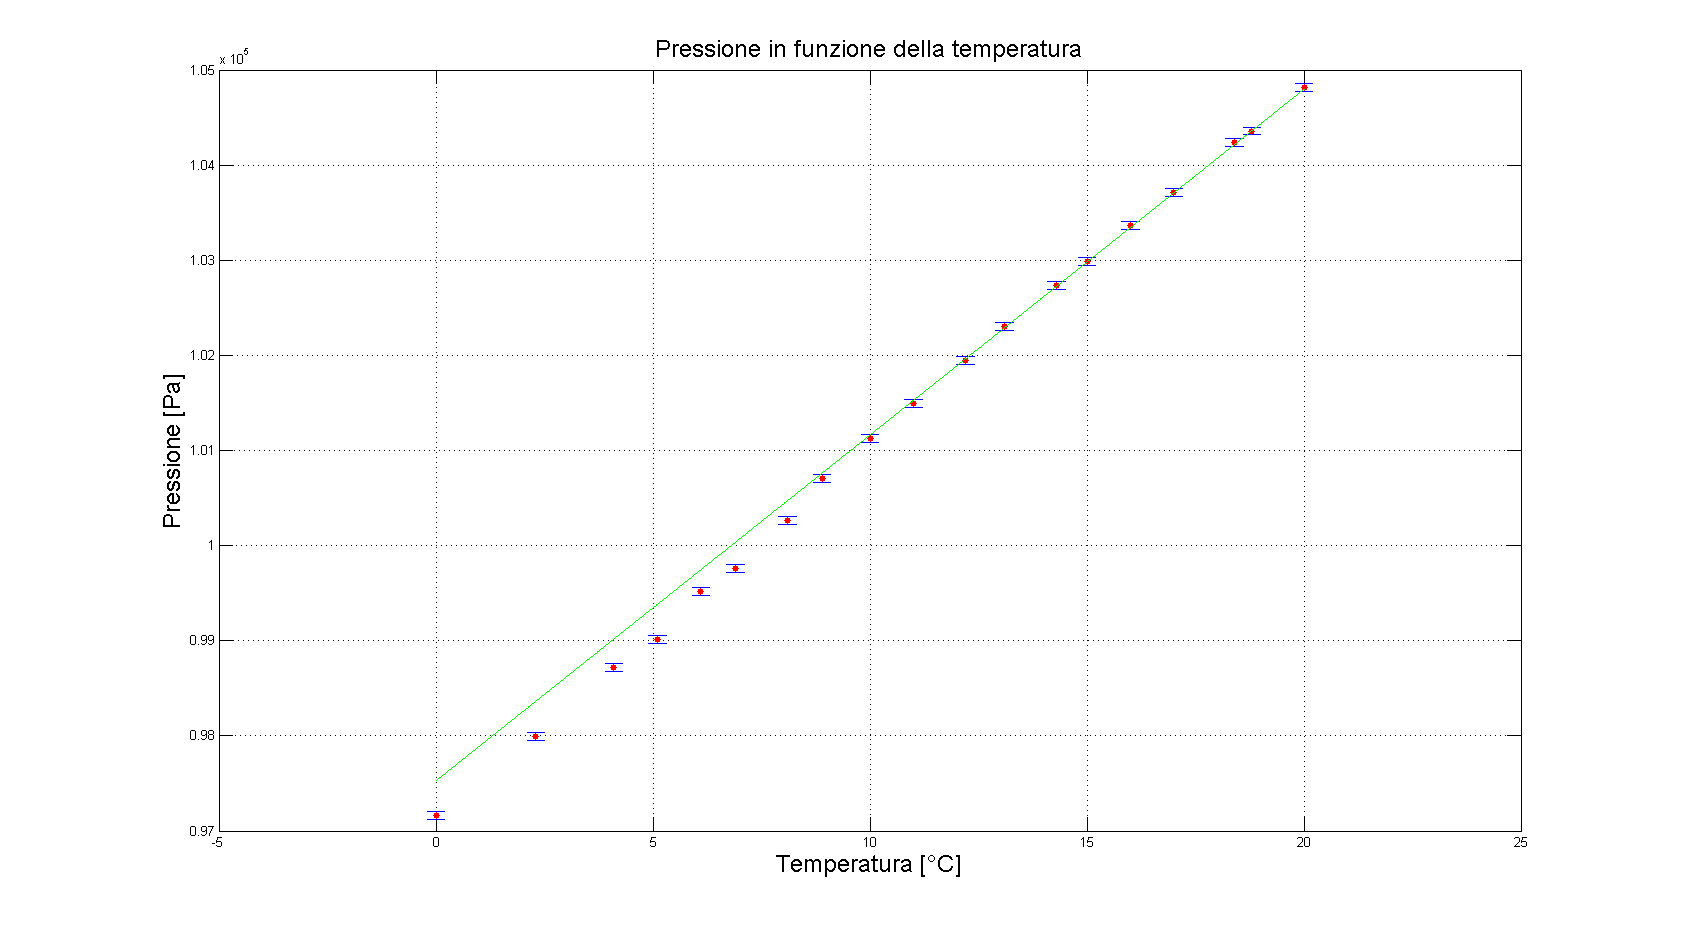
\includegraphics[width=\textwidth]{img/3}
\caption{Grafico a barre della pressione $P$ in funzione della temperatura}
\end{figure}

In Figura 3 si nota il diverso comportamento della pressione al di sotto della temperatura di rugiada, per calcolare lo zero assoluto possiamo quindi utilizzare solamente i dati più affidabili, ovvero quelli al di sopra di tale temperatura.
Il dislivello $h$ è legato in maniera lineare alla temperatura, pertanto:
\begin{equation}
\rho gh = \rho g (A + B T)
\end{equation}
con A e B costanti.
Ma allora dalla \eqref{eq:p} otteniamo che:
\begin{equation}
P = P_A + \rho g (A + B T) = f (T)
\end{equation}
dove $f(T)$ sarà la retta da considerare per la determinazione dello zero assoluto.
Infatti lo zero assoluto $T_0$ è rappresentato graficamente dall'intersezione dell'asse delle ascisse, ovvero $P = 0$, e la funzione $f(T)$.
Quindi lo zero assoluto vale: 
\begin{equation}
T_0 = \frac{P_A - A \rho g}{\rho gB} = -2.7 K
\end{equation}

SI VALUTI L'INCERTEZZA SU $T_0$ DOVUTA ALLA PROPAGAZIONE DELL'INCERTEZZA SULLE GRANDEZZE MISURATE DIRETTAMENTE.